In figure \ref{fig:elfi-model} we present an overview of our
implementation; one could think of figure~\ref{fig:elfi-model} as a
depiction of the main class of our implementation, which is called
ROMC, while the entities inside the green and blue ellipses are the
main functions of the class. Following the common naming principles,
the methods starting with an underscore (green ellipses) represent
internal (private) functions and are not meant to be used by a user,
whereas the rest of the methods (blue ellipses) are the
functionalities used for performing the inference.As mentioned before,
the implementation favours extensibility; the building blocks that
compose the method have been designed in an isolated fashion so that a
practitioner may replace them without the method to collapse.

Figure \ref{fig:elfi-model} groups the ROMC implementation into the
training, the inference and the evaluation part, following the
arrangement used in the algorithmic presentation (section
\ref{subsec:romc-algorithmic}). The training part includes all the
steps until the computation of the proposal regions; sampling the
nuisance variables, defining the optimisation problems, solving them
and constructing the regions. The inference part comprises of
evaluating the unnormalised posterior (and the normalised one, in
low-dimensional cases), sampling and computing an
expectation. Moreover, the ROMC implementation provides some utilities
for inspecting the training process, such as plotting the histogram of
the distances
$d^*_i = g_i(\theta_i^*), \: \forall i \in \{1, \ldots, n_1
\}$ after solving the optimisation problems and visualising the
constructed bounding box\footnote{if the parametric space is up to
  $2D$}. Finally, there are implemented two functionalities for
evaluating the inference; (a) computing the Effective Sample Size
(ESS) of the obtained weighted samples and (b) measuring the
divergence of the approximate posterior from the ground-truth, if the
latter is available.\footnote{Normally, the ground-truth posterior is
  not available; that is the meaning of performing the inference!
  Though this functionality is useful in cases where the posterior can
  be computed numerically or with an alternative method (i.e.\ ABC
  Rejection Sampling) and we would like to measure the discrepancy
  between the two approximations.}


\subsubsection*{Simple 1D example}

For illustrating the implemented functionalities, we choose the
following $1D$ as as in
\cite{Ikonomov2019}; the prior distribution is the uniform in the
range $[-2.5, 2.5]$, i.e.\ $p(\theta) = \mathcal{U}(\theta;-2.5,2.5)$
and the generative model is the following,

\begin{gather} \label{eq:1D_example}
  p(y|\theta) = 
  \left\{
    \begin{array}{ll}
      \theta^4 + u & \mbox{if } \theta \in [-0.5, 0.5] \\
      |\theta| - c + u & \mbox{otherwise} 
    \end{array} \right.
\end{gather}

\noindent
where $u \sim \mathcal{N}(0,1)$. There is only one observation
$y_0 = 0$. In this example, the likelihood can be evaluated quite
easily, hence it can be solved quite easily without a likelihood-free
inference model. This is quite convenient at this point, since apart
from illustrating the functionalities, we can quite easily validate
the inference. The ground-truth posterior of the example is shown in
figure \ref{fig:example_gt}.

\begin{figure}[h]
    \begin{center}
      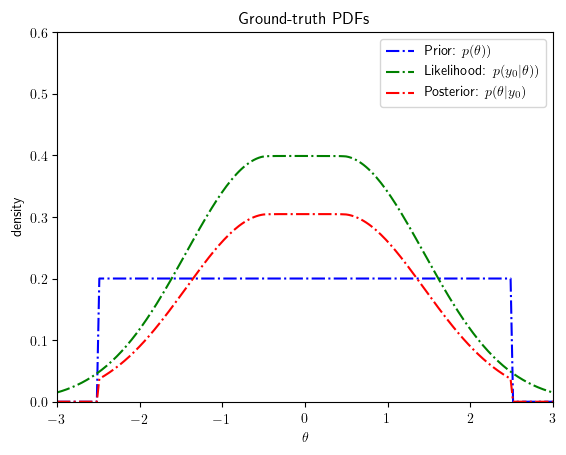
\includegraphics[width=0.5\textwidth]{./Thesis/images/chapter3/example_gt.png}
    \end{center}
  \caption{Ground-truth posterior distribution for our simple 1D example}
  \label{fig:example_gt}
\end{figure}

The corresponding \textit{elfi} code for building the specific generative model is the following.

\subsubsection*{ELFI code for modelling the example}

In the following code snippet, we model the simple example in the ELFI
package. We observe that the initialisation of the ROMC inference
method is quite intuitive; we juct pass the distance node of the
simulator as the first argument. The arguments \pinline{left_lim,
  right_lim} which represent the limits of the prior distribution are
optional; they are needed only if \pinline{romc.eval_posterior()} is
called in the inference part, for approximating the partition.

\begin{pythoncode}
  import elfi
  import scipy.stats as ss
  import numpy as np
  
  def simulator(t1, batch_size=1,random_state=None):
      if t1 < -0.5:
          y = ss.norm(loc=-t1-c, scale=1).rvs(random_state=random_state)
      elif t1 <= 0.5:
          y = ss.norm(loc=t1**4, scale=1).rvs(random_state=random_state)
      else:
          y = ss.norm(loc=t1-c, scale=1).rvs(random_state=random_state)
      return y

  # observation
  y = 0
      
  # Elfi graph    
  t1 = elfi.Prior('uniform', -2.5, 5)
  sim = elfi.Simulator(simulator, t1, observed=y)
  d = elfi.Distance('euclidean', sim)

  # Define ROMC inference method
  left_lim = np.array([-2.5])
  right_lim = np.array([2.5])
  romc = elfi.ROMC(d, left_lim=left_lim, right_lim=right_lim)
\end{pythoncode}


\begin{figure}[!ht]
    \begin{center}
      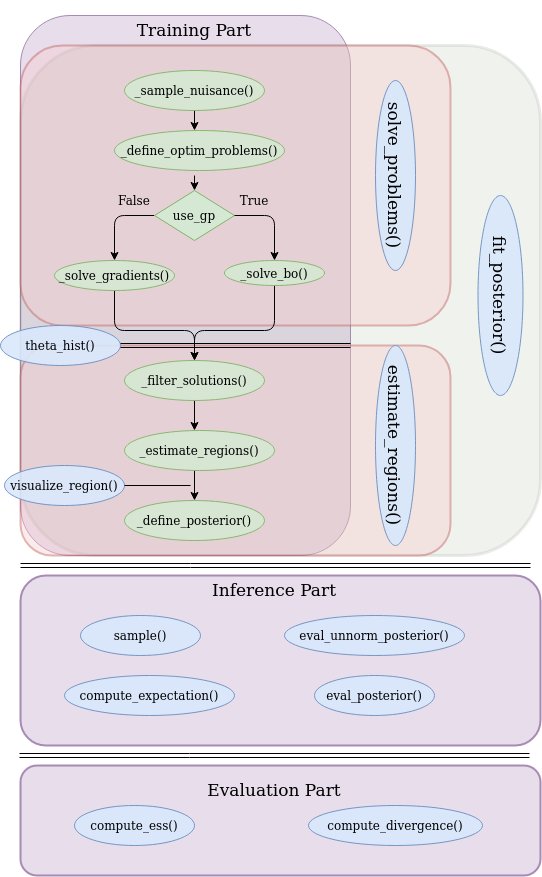
\includegraphics[width=0.75\textwidth]{./Thesis/graphs/ROMC.png}
    \end{center}
    \caption{Overview of the ROMC implementation. The training part
      follows a sequential pattern; the functions in the green
      ellipses must be called in a sequential fashion for completing
      the training part and define the posterior distribution. The
      functions in blue ellipses are the functionalities provided to
      the user.}
    \label{fig:elfi-model}
\end{figure}

  